
\begin{IEEEbiography}[{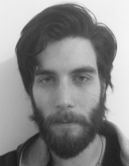
\includegraphics[width=1in,clip,keepaspectratio]{img/brice.png}}]
{Brice N{\'e}delec} He received his M.Sc. degree in Software Architecture from
the University of Nantes (France) in 2012, and his Ph.D. in computer science
from the University of Nantes in 2016. He currently holds a post-doctoral
position in the team GDD (Distributed Data Management). His main research
interests include, but are not limited to, distributed applications,
collaborative tools, causality tracking, consistency criteria, and distributed
networks. Overall, he is just interested in solving puzzling problems.
\end{IEEEbiography}

\begin{IEEEbiography}[{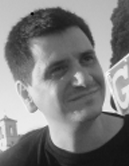
\includegraphics[width=1in,clip,keepaspectratio]{img/pascal.png}}]
{Pascal Molli} He graduated from Nancy University (France) and received his
Ph.D. in computer science from Nancy University in 1996.  From 1997 to September
2010, he has been Associate Professor at University of Nancy. He participated to
the creation of the INRIA ECOO (Environments for Cooperation) project. In 2001,
he became vice-head of the INRIA ECOO Team. In October 2009, he created and led
the INRIA SCORE team. From September 2010 to current, he is Full Professor at
University of Nantes and is head of GDD Team in LS2N research center.  Pr. Molli
mainly worked on collaborative distributed systems and focused on problems of
consistency of shared data in collaborative environments and awareness models
for collaborative editing. His current research topics are
\begin{inparaenum}[(i)]
\item algorithms for distributed collaborative systems: consistency criteria for
collaborative systems and algorithms to enforce consistency;
\item Collaborative distributed systems for the Semantic Web: How to allow people 
and computers to edit concurrently the web and the semantic web?
\end{inparaenum}
\end{IEEEbiography}


\begin{IEEEbiography}[{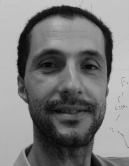
\includegraphics[width=1in,clip,keepaspectratio]{img/achour.png}}]
{Achour Most{\'e}faoui} He received his M.Sc. degree in computer science in
1991, and a Ph.D. in computer science in 1994 both from the University of
Rennes. He has been Associate Professor in the Computer Science of the
University of Rennes from 1996 to 2011 when he joined the University of Nantes
as full professor.  He spent one semester in the Theory of Computing group of
the CSAIL Lab. in the Massachusetts Institute of Technology in 2007.  Since
September 2011, he is head of a Master's diploma in Computer Science (University
of Nantes) and he is co-head of the GDD research team within the LS2N research
center.  His research interests are on distributed computing: agreement and
calculability issues in asynchronous, fault-prone distributed systems and
replicated data structures.  More specifically, he is interested in discovering
the boundary between solvable and unsolvable tasks and, understanding further
assumptions/relaxations needed to solve otherwise impossible tasks.  A second
direction is to study replicated date structure (queue, tuple space,
transactional memory, wiki, etc.).  How to specify and implement distributed
data structures and then integrate them into programming languages in different
distributed computing models. For both directions, distributed algorithms design
is the key point in my work, either to study algorithmic mechanisms, to
efficiently solve tasks, or to show impossibility results through reductions.
\end{IEEEbiography}

%%% Local Variables:
%%% mode: plain-tex
%%% TeX-master: "../paper"
%%% End:
